%************************************************
\chapter{User Guide}\label{ch:user_guide} % $\mathbb{ZNR}$
%************************************************

The application provides five functions:

\begin{itemize}
\item Requesting and displaying web-pages.
\item Managing the history of requested web-pages.
\item Managing user-defined favourites.
\item Managing a user-defined home-page.
\item Allow printing of the currently displayed web-page.
\end{itemize}

These functions shall be explained in this chapter.

\section{Requesting a web-page}
\label{sec:request_web_page}

Upon starting the application the user will see the following window:

\begin{figure}[H]
\begin{center}
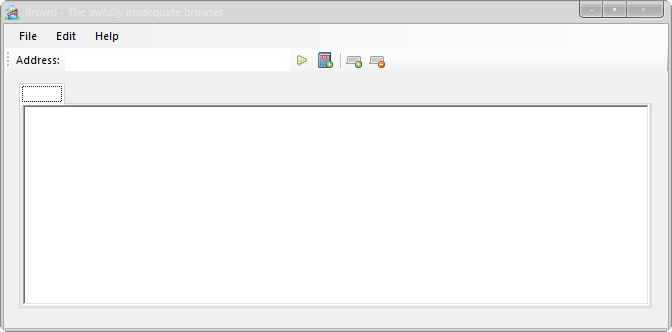
\includegraphics[width=\textwidth]{gfx/main_window.png}
\caption{The application's main window.}
\label{fig:main_window}
\end{center}
\end{figure}

To request a web-page the user must enter the desired address in the \texttt{Address} text-box and then press the \texttt{Go}-button (\raisebox{-1mm}{
\includegraphics{gfx/16-arrow-right.png}}).

The format of the entered address will be verified. It must match the following pattern\footnote{Parts in square-brackets may not be required for all web-pages.}:

\begin{lstlisting}[language=xml]
http://[www.]address.domain[/url-path]
\end{lstlisting}

Should the entered address not match the given format, the program will notify the user about the error by displaying a message-box:

\begin{figure}[H]
\begin{center}
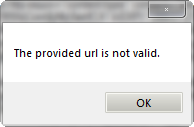
\includegraphics[scale=1]{gfx/error_message.png}
\caption{Error message due to invalid url.}
\label{fig:error_message}
\end{center}
\end{figure}

When the url is valid the browser will display the \ac{HTML}-code in the current tab:

\begin{figure}[H]
\begin{center}
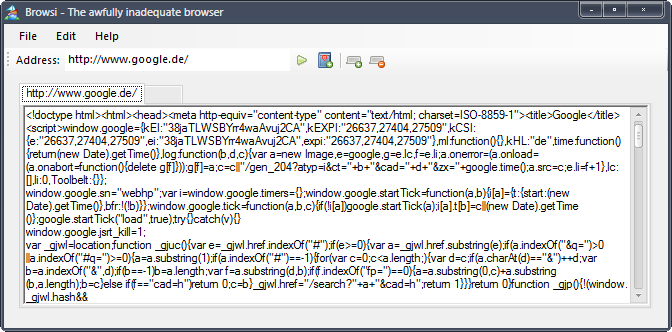
\includegraphics[width=\textwidth]{gfx/display_page.png}
\caption{Browser displaying the current web-page.}
\label{fig:display_page}
\end{center}
\end{figure}

To request multiple pages simultaneously it is possible to utilize tabs:

To create a new tab, the user simply presses the \texttt{AddTab}-button (\raisebox{-1mm}{
\includegraphics{gfx/tab_add.png}}). This will create new (and empty) tab-page.

Should the user want to close a tab it is necessary to select the tab that should be closed and the press the \texttt{RemoveTab}-button (\raisebox{-1mm}{
\includegraphics{gfx/tab_delete.png}}).
